% =====================================================================
%  Chapitre 2 -- partie b : echelle, outliers, pipeline, fuite
% =====================================================================

\begin{frame}{Mettre à l'échelle : pourquoi c'est vital}
\begin{columns}[t]
\begin{column}{0.46\textwidth}
\centering
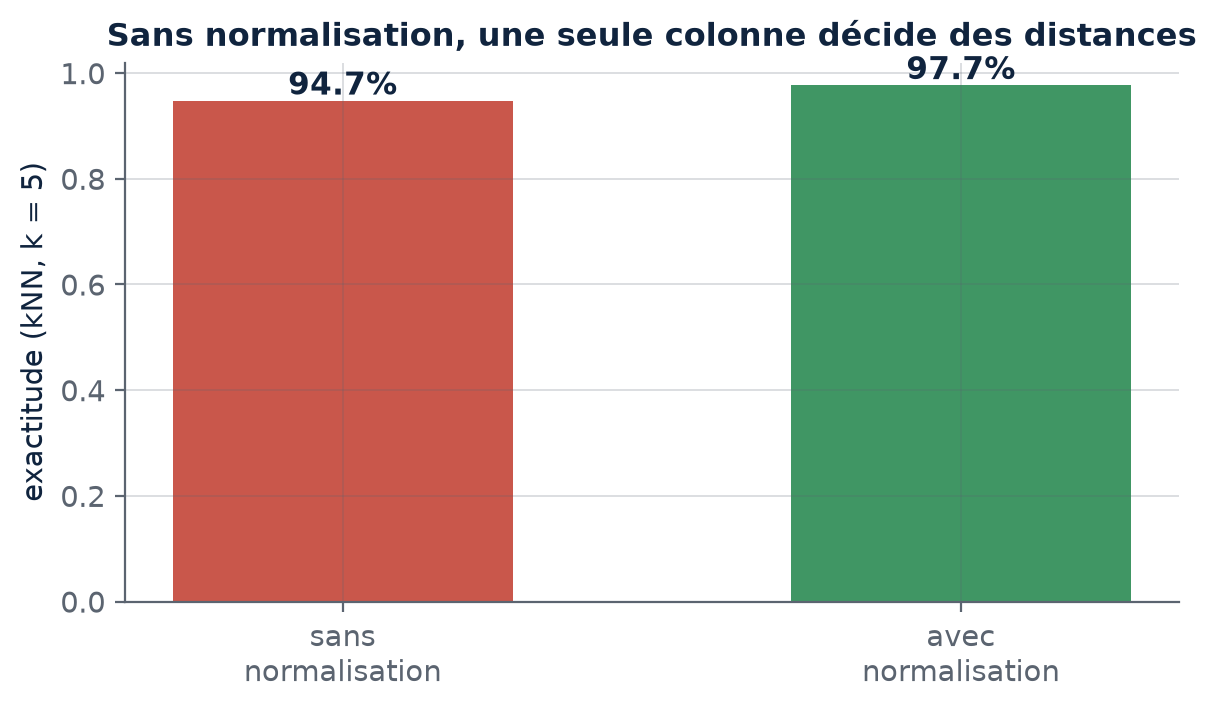
\includegraphics[height=0.32\textheight,keepaspectratio]{h04_echelle.png}
\end{column}
\begin{column}{0.52\textwidth}
\begin{wbox}[Le rapport des étendues]
Sur ce jeu, la colonne la plus large couvre $4\,069$ unités, la plus étroite
$0{,}029$ : un rapport de \textbf{140\,569}.
\end{wbox}
\begin{itemize}
  \item kNN sans normalisation : \textbf{94,7 \%}.
  \item avec normalisation : \textbf{97,7 \%} --- \textbf{+2,9 points}.
  \item Méthodes à \textbf{distances} concernées : kNN, SVM, k-means.
  \item Les \textbf{arbres} y sont insensibles (seuils, pas distances).
\end{itemize}
\end{column}
\end{columns}

\end{frame}

\begin{frame}{Trois mises à l'échelle, trois usages}
\begin{center}
\small
\begin{tabular}{@{}p{0.20\textwidth}p{0.36\textwidth}p{0.34\textwidth}@{}}
\toprule
\textbf{Méthode} & \textbf{Formule} & \textbf{Quand} \\
\midrule
Standardisation & $(x-\mu)/\sigma$ & par défaut ; suppose une dispersion
stable \\
Normalisation min-max & $(x-\min)/(\max-\min)$ & bornes connues, réseau de
neurones \\
Mise à l'échelle robuste & $(x-\text{médiane})/\mathrm{IQR}$ & présence
d'outliers \\
\bottomrule
\end{tabular}
\end{center}
\vspace{1.5mm}
\begin{wbox}[Ce qui doit être appris sur l'entraînement seul]
$\mu$, $\sigma$, $\min$ et $\max$ sont des \textbf{paramètres} estimés sur les
données. Les calculer sur l'ensemble revient à faire entrer le test dans
l'entraînement.
\end{wbox}
\end{frame}

\begin{frame}{Valeurs aberrantes : deux détections, deux résultats}
\begin{columns}[t]
\begin{column}{0.52\textwidth}
\centering
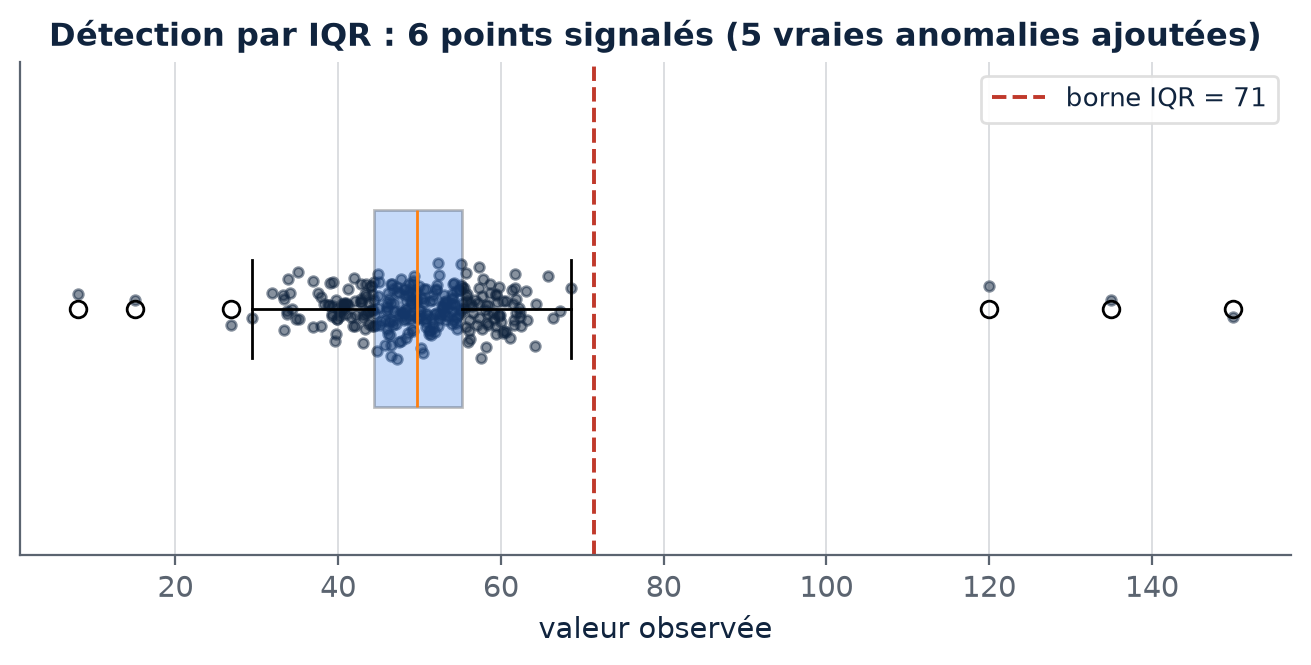
\includegraphics[height=0.34\textheight,keepaspectratio]{h05_outliers.png}
\end{column}
\begin{column}{0.44\textwidth}
\begin{itemize}
  \item \textbf{IQR} : signalé si $x < Q_1 - 1{,}5\,\mathrm{IQR}$ ou
        $x > Q_3 + 1{,}5\,\mathrm{IQR}$. Ici : \textbf{6 points}.
  \item \textbf{Z-score} : $|z| > 3$. Ici : \textbf{4 points}.
  \item 5 anomalies avaient été ajoutées : aucune règle ne les retrouve
        toutes.
\end{itemize}
\begin{kbox}[Conséquence]
La détection d'outliers est un choix de seuil, pas une vérité. On le justifie
et on le documente.
\end{kbox}
\end{column}
\end{columns}
\end{frame}

\begin{frame}{Que faire d'une valeur aberrante ?}
\begin{center}
\small
\begin{tabular}{@{}p{0.24\textwidth}p{0.34\textwidth}p{0.34\textwidth}@{}}
\toprule
\textbf{Situation} & \textbf{Action} & \textbf{Justification} \\
\midrule
Erreur de saisie & corriger ou supprimer & 1\,575 °C est physiquement
impossible \\
Valeur réelle extrême & conserver, changer de perte & un revenu très élevé
existe \\
Mesure influente & winsoriser (borner) & on garde l'ordre sans le poids
excessif \\
\bottomrule
\end{tabular}
\end{center}
\vspace{1.5mm}
\begin{wbox}[Ne jamais supprimer sans regarder]
Supprimer les 5 \% de valeurs les plus hautes d'un revenu, c'est supprimer les
5 \% de ménages les plus riches --- et fausser toute conclusion économique.
\end{wbox}
\end{frame}

\begin{frame}{Discrétiser : quand et pourquoi}
\begin{columns}[t]
\begin{column}{0.48\textwidth}
\begin{ebox}[Quand c'est utile]
\begin{itemize}
  \item relation manifestement non linéaire (âge et risque) ;
  \item beaucoup de valeurs identiques ou arrondies ;
  \item besoin d'interprétation par tranches.
\end{itemize}
\end{ebox}
\end{column}
\begin{column}{0.48\textwidth}
\begin{wbox}[Quand c'est une faute]
\begin{itemize}
  \item on perd de l'information ;
  \item les frontières sont arbitraires ;
  \item un modèle à arbres fait déjà ce découpage tout seul.
\end{itemize}
\end{wbox}
\end{column}
\end{columns}
\vspace{1.5mm}
\begin{kbox}[Règle]
Discrétiser est un choix de modélisation, pas une étape obligatoire. On le
justifie par une hypothèse, pas par confort.
\end{kbox}
\end{frame}

\begin{frame}{Tout mettre dans un pipeline}
\begin{center}
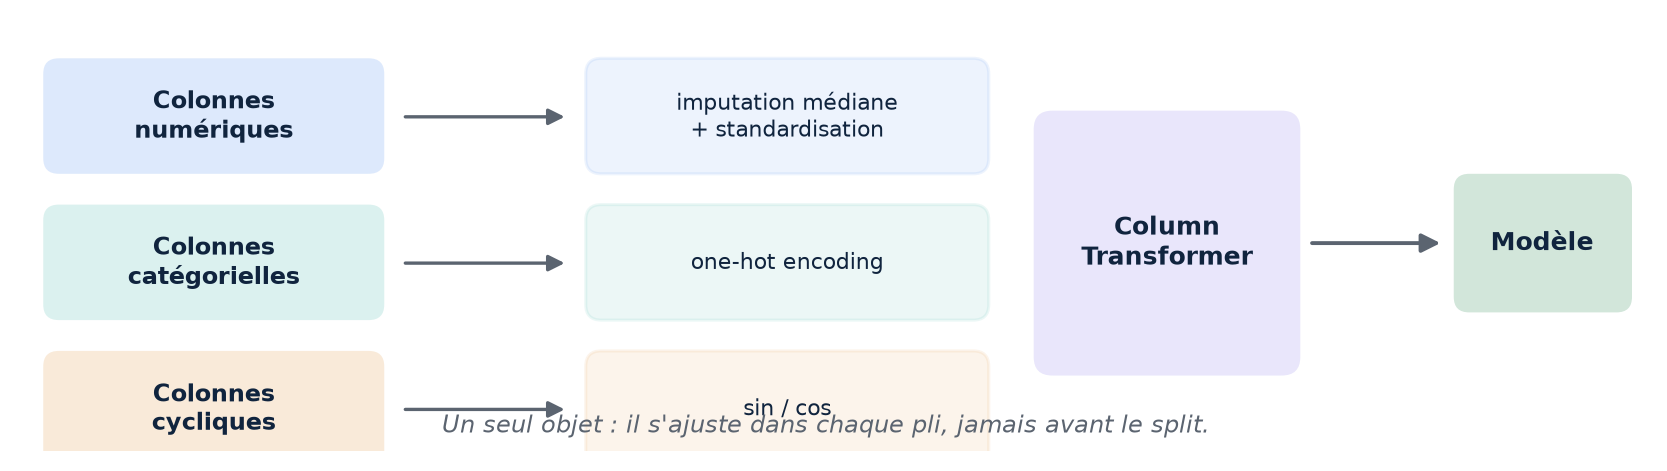
\includegraphics[width=0.95\textwidth]{h07_pipeline.png}
\end{center}
\vspace{1mm}
\begin{columns}[t]
\begin{column}{0.48\textwidth}
\footnotesize
\textbf{Un objet unique} qui contient l'imputation, l'encodage et la mise à
l'échelle. Il s'ajuste avec \py{fit} sur l'entraînement, s'applique avec
\py{transform} sur le test.
\end{column}
\begin{column}{0.48\textwidth}
\footnotesize
\textbf{Conséquence} : dans chaque pli de validation croisée, les paramètres
de prétraitement sont réestimés. C'est la seule façon d'éviter la fuite.
\end{column}
\end{columns}
\end{frame}

\begin{frame}{La fuite par encodage cible}
\begin{columns}[t]
\begin{column}{0.44\textwidth}
\centering
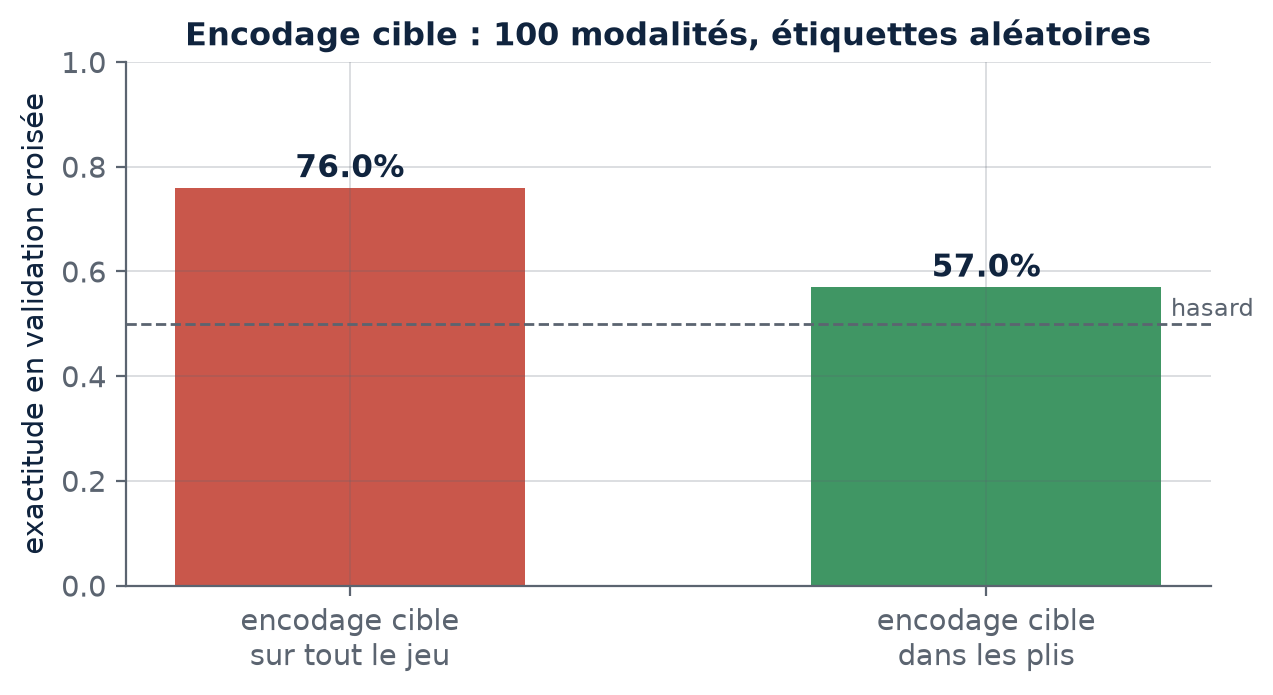
\includegraphics[height=0.34\textheight,keepaspectratio]{h06_fuite_encodage.png}
\end{column}
\begin{column}{0.54\textwidth}
\begin{itemize}
  \item 100 modalités, 2 lignes chacune, étiquettes \textbf{aléatoires}.
  \item Encodage calculé sur tout le jeu : \textbf{76,0 \%}.
  \item Encodage recalculé dans chaque pli : \textbf{57,0 \%}.
  \item Écart : \textbf{+19 points} pour rien.
\end{itemize}
\begin{wbox}[Mécanisme]
Avec deux lignes par modalité, la moyenne de $y$ dans la modalité contient
l'étiquette de la ligne elle-même : la variable encode la réponse.
\end{wbox}
\end{column}
\end{columns}
\end{frame}

\begin{frame}{Activité 2 --- trouver la fuite (8 min)}
\begin{abox}[Trois pipelines. Lequel est correct ?]
\begin{enumerate}
  \item \py{StandardScaler().fit(X)} puis \py{train_test_split}.
  \item \py{imputer.fit_transform(X_train)} puis transformation du test avec
        le même imputer.
  \item Encodage cible calculé sur \py{X_train} avant la validation croisée.
\end{enumerate}
\end{abox}
\vspace{1mm}
\begin{solbox}[Réponses]
\textbf{1.} Faux : les paramètres voient le test.
\textbf{2.} Correct : ajustement sur l'entraînement, application au test.
\textbf{3.} Faux : l'encodage doit être refait dans chaque pli.
\end{solbox}
\end{frame}

\begin{frame}{Étude de cas : le prétraitement qui gonfle le score}
\begin{wbox}[La situation]
Un groupe annonce \textbf{89 \%} de rappel sur la détection de fraude. Son
notebook fait, dans cet ordre :
\begin{enumerate}
  \item suppression des lignes incomplètes sur tout le jeu ;
  \item \py{StandardScaler} ajusté sur tout le jeu ;
  \item encodage cible de la variable « agence » (120 modalités) ;
  \item découpage 80/20 et entraînement.
\end{enumerate}
\end{wbox}
\vspace{1mm}
\begin{abox}[À traiter en binôme (10 min)]
Quelles étapes fuient, et dans quel ordre refaire le pipeline ?
Quel score vous attendez-vous à obtenir réellement ?
\end{abox}
\end{frame}

\begin{frame}{Quiz 2 --- échelle, outliers, pipeline}
\begin{columns}[t]
\begin{column}{0.49\textwidth}
\begin{qbox}[Question 1]
Quel modèle est insensible à l'échelle ?
\begin{itemize}
  \item[(a)] kNN \quad (b) forêt aléatoire \quad (c) SVM à noyau
\end{itemize}
\end{qbox}
\begin{qbox}[Question 2]
La borne haute d'IQR vaut :
\begin{itemize}
  \item[(a)] $Q_3 + 1{,}5\,\mathrm{IQR}$ \quad (b) $\mu + 3\sigma$
  \item[(c)] le maximum
\end{itemize}
\end{qbox}
\end{column}
\begin{column}{0.49\textwidth}
\begin{qbox}[Question 3]
Où doit être ajusté un \py{StandardScaler} ?
\begin{itemize}
  \item[(a)] sur tout le jeu, avant le split
  \item[(b)] sur l'entraînement, dans le pipeline
  \item[(c)] sur le test
\end{itemize}
\end{qbox}
\begin{solbox}[Réponses]
\textbf{1.} (b). \quad \textbf{2.} (a). \quad \textbf{3.} (b).
\end{solbox}
\end{column}
\end{columns}
\end{frame}
